\section{Multigrid}

O principal custo computacional que simulações CFD possuem, quando os métodos de projeção para o acoplamento pressão-velocidade são usados, é a solução da equação elíptica de Poisson para a pressão. Essa equação é objeto de estudo de diversos grupos, por ser a de mais difícil convergência e geralmente representar o maior gargalo nas simulações. Diversas técnicas foram desenvolvidas para lidar com esse problema, entre elas destacam-se os métodos de Krylov e o multigrid. 

O multigrid é um método de solução de sistemas lineares, introduzido para lidar com a natureza das equações elípticas. Foi apresentado pela primeira vez por \citet{Fedorenko1962} e expandido pelo mesmo em \citet{Fedorenko1964}, porém o método só passou a ser utilizado amplamente como ferramenta mais tarde, com trabalhos como o de \cite{Brandt1977}, que generalizou o método para problemas não lineares e refinamento local.

O método consiste em utilizar várias malhas, cada vez mais grosseiras, para resolver o sistema de equações lineares criado pela discretização da equação de Poisson. Ele se baseia na propriedade de que alguns solvers iterativos clássicos, como Jacobi e Gauss-Seidel, eliminam em poucas iterações componentes de alta frequência do erro, enquanto a convergência estagna nas componentes de baixa frequência. Uma componente de baixa frequência em uma malha de espaçamento $h$ passa a ser de alta frequência em uma malha de espaçamento $2h$, podendo ser eliminada a um custo menor, dado que as malhas grosseiras possuem matrizes menores. Como o erro associado ao sistema linear é difícil de ser obtido em problemas numéricos no geral, utiliza-se o resíduo do sistema como parâmetro de medida. Sendo assim, uma equação residual é resolvida em cada nível, Eq. \ref{eq:multigrid_res}:

\begin{equation}
    A\Delta x = r,
    \label{eq:multigrid_res}
\end{equation}

na qual $A$ é a matriz dos coeficientes, $r = b - A\tilde{x}$ o resíduo e $\Delta x$ pode ser definido como: dado o sistema $Ax = b$ e uma aproximação para o sistema linear $\tilde{x}$ em que $\Delta x = x - \tilde{x}$, $\Delta x$ atende a Eq. \ref{eq:multigrid_res}.

Assim os resíduos $r$ dos níveis superiores são transferidos para os níveis inferiores, em uma operação chamada de restrição. Após os cálculos nos níveis inferiores amortecerem as altas frequências, a correção $\Delta x$ é adicionada à solução dos níveis superiores em um movimento chamado de prolongação, seguida de uma nova suavização com iterações do suavizador. Esse processo se repete em ciclo. Por não resolverem o sistema em si, mas apenas suavizá-lo, os métodos de solução de sistemas lineares utilizados aqui são chamados de suavizadores (\textit{Smoothers}).


Os níveis podem se comunicar de diversas formas, sendo esse um dos objetos de estudo do tema, a Figura \ref{fig:cycles} ilustra alguns dos mais utilizados, sendo que os ciclos se diferenciam principalmente pela forma com que realizam restrições e prolongações.

\begin{figure}
    \centering
    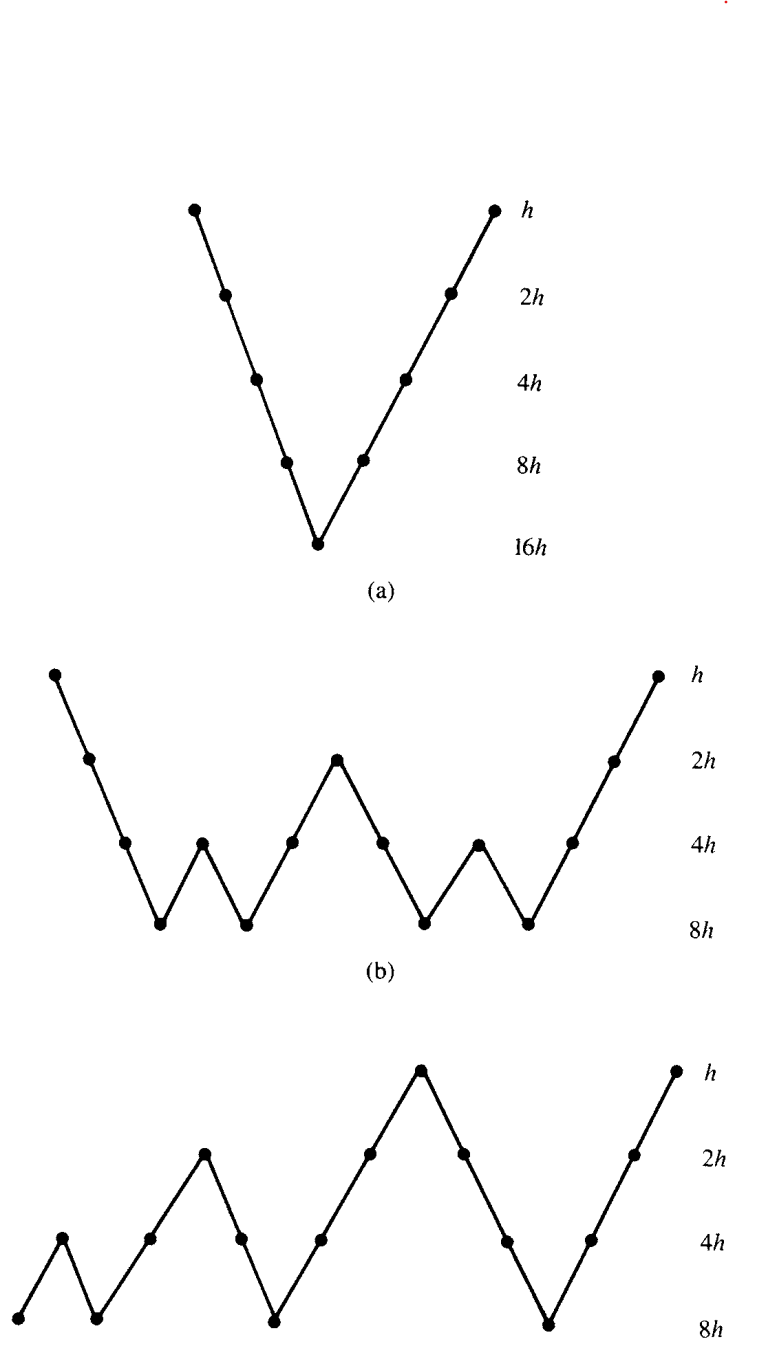
\includegraphics[width = 0.6\textwidth]{imagens/cycles.png}
    \caption{Representação das diversas possibilidades de ciclos para o multigrid. (a) representando o V-cycle (b) representando o W-cycle e (c) representando o esquema FMG. Fonte: \citet{Briggs2000}}
    \label{fig:cycles}
\end{figure}

Na figura \ref{fig:cycles} é possível observar três formas de se realizar as restrições e prolongamentos. O V-cycle, que consiste em uma descida sequencial de restrições até o nível mais inferior, com um número de iterações dos suavizadores sendo realizado a cada nível, seguido de uma subida também sequencial de prolongações, nas quais mais ciclos dos suavizadores são realizados. o W-cycle dobra o número de vezes que cada nível realiza a restrição, dobrando o número de estimativas de erro a cada nível mais grosseiro, o que melhora a estimativa do erro, porém deixa o método mais caro. o full Multigrid (FMG) é um conjunto de iterações aninhadas, resolvendo o problema todo - e não apenas a estimativa do resíduo - nos níveis mais grosseiros utilizando o multigrid e entregando o resultado dessa solução a níveis mais finos de forma interpolada.

Existem duas formas clássicas abordadas na literatura para se realizar a representação dos níveis auxiliares utilizados para o multigrid, uma delas é guardá-los diretamente na memória e discretiza a equação resolvida para obter a matriz A diretamente em cada nível, o que garante um menor custo computacional em malha estruturada, esse método é chamado de multigrid geométrico. A outra abordagem é o chamada multigrid algébrico que consiste em construir os componentes na matriz A da malha mais fina original a partir de produtos de matrizes. Este último método consome mais memória e tende a ser utilizado em malhas não estruturadas. 

O multigrid geométrico implementado por \citet{Villar2007} é utilizado no presente trabalho para a resolução da pressão no escoamento principal, o código utiliza um ciclo em V e (verificar) como suavizador, com o critério de parada definido como (verificar). Uma explicação mais abrangente em relação a como a hierarquia de malha do código utiliza tanto o multigrid quanto o AMR é realizada na Seção \ref{sec:hierarquia}.
